\documentclass[a4paper,12pt]{article}

\setlength{\textwidth}{15.0cm}
\setlength{\textheight}{24.0cm}
\setlength{\topmargin}{0cm}
\setlength{\headsep}{0cm}
\setlength{\headheight}{0cm}
\pagestyle{plain}

\usepackage[style=alphabetic,backend=biber]{biblatex} 
\addbibresource{bibliography.bib}

\usepackage{amsmath, amsfonts, mathtools, amsthm, amssymb}
\usepackage{import}
\usepackage{pdfpages}
\usepackage{transparent}
\usepackage{xcolor}
\setlength{\parindent}{0pt}


% \renewcommand{\bibfont}{\footnotesize}


\title{The use/abuse of copulas in actuarial science and finance}
\date{}

\begin{document}
\maketitle

\begin{abstract}
    This is an assignment for the actuarial models course.
    The assignment is to summarize \cite{dempster_correlation_2002}, \cite{frees_understanding_1998},
    \cite{donnelly_devil_nodate} and discuss the following:

    \begin{itemize}
        \item  The purpose is to understand the impact of the assumption regarding
              the dependence structure between risk factors.
        \item  This is done by means of the concept of copulas.
        \item  In particular, we study the impact of misused copulas and correlation in the
              valuation of collateralized debt obligations (CDO's).
    \end{itemize}

\end{abstract}

\section{Overview}
\cite{dempster_correlation_2002} introduces linear dependency, copulas, comonotonicity and rank correlation which
already are introduced in the course. Also spherical/elliptical distributions and tail dependence are introduced.
Spherical/elliptical distributions generalize the normal distribution and has good properties for common dependency
measures.  Tail dependence quantifies dependency in the tails. They also discuss some
common dependency fallacies and simulation of copulas.\\

\cite{frees_understanding_1998} also introduces copulas, present examples, simulation
and fitting of copulas. Fitting copulas is done by choosing a parametric model
guided by non-parametric density estimation and parametric estimation is done
with MLE and AIC.
Main examples are joint mortality modeling and modeling insurance company indemnity claims.
And finally also introducing stochastic orders and distortion functions which we also covered previously. \\

\cite{donnelly_devil_nodate} also introduces copulas but primarily focuses on the 2007-2008 financial crisis.
It mainly discusses modeling Collateralized Debt Obligations (CDOs) and trenching, the impact of
incorrectly modeling dependence, highlighting the consequences of incorrectly modelling default clustering.
This is illustrated through an example of modeling the default probability of bonds under the assumption
of identical pairwise correlation. \\

\cite{lopez-paz_dependence_2016} is a phd thesis we like with a section on copulas. It introduces
the empirical copula transformation we use later in Figure \ref{fig:pair plot psuedo copula}. \\


\section{Introduction to new concepts}

\subsection{Spherical/elliptical distributions}
Spherical/elliptical distributions have a spherical/elliptical symmetry. I.e.
we can characterize a spherical distributions $X$ as follows:
\begin{equation}
    X =_{d} R U
    .
\end{equation}
with $R$ a positive random variable and $U$ independent of $R$ a random vector uniformly distributed on the unit sphere.
Elliptical distributions can be obtained as affine transformations of spherical distributions. Elliptical distributions
are fully characterized by their mean, covariance matrix and the characteristic function of normalized $R$
(normalize such that the mean $=1$) also called generator when the covariance exists ($E[R^{2}]<\infty$).
So it is a semi-parametric family of distributions with
limited $1$ dimensional non-parametric random variable.  \\

Here are some obvious properties of elliptical distributions:
\begin{itemize}
    \item An affine transformation of an elliptical distribution is also elliptical.
    \item The sum in the set of elliptical distributions with the same generator is closed.
    \item Marginal and conditional  distributions of the components of elliptical distributions are elliptical. The intuition
          for this is the same as for normal distributions, the intersection between ellipsoids and planes are also ellipsoids.
\end{itemize}

In \cite{dempster_correlation_2002} they show that linear portfolios where individual risk together are jointly elliptical
distributed, risk measures lose structure, simplifying risk management tasks. Specifically they show that VaR is equivalent
to variance risk analysis. This emphasizes that the assumption of elliptical distributions is a strong assumption and
normal distributions are even stronger.

\subsection{Tail dependence}
Making assumptions is dangerous. Data trades-off with assumptions.
Determining high dimensional structure non-parametrically requires a lot of data.
Dependence is a high dimensional structure and at
tails we have little data both by definition. So naturally making
assumptions about the dependence structure at the tails is essential.
Tail dependence is a way to quantify the dependence in the tails .
The upper tail dependence ($\lambda$) between $X$ and $Y$ is defined as follows:
\begin{equation}
    \lim_{\alpha \to 1-}  P[ Y > F_{2}^{-1} ( \alpha) \mid X > F_{1}^{-1} ( \alpha) ]=\lambda.
\end{equation} \\
When $X$ and $Y$ are continuous distribution we can express this in terms
of their copula:

\begin{align}
     & \lim_{\alpha \to 1-}  P[ Y > F_{2}^{-1} ( \alpha) \mid X > F_{1}^{-1} ( \alpha) ]                                          \\
     & =\lim_{\alpha \to 1-}  P[ U_{2} >  \alpha \mid U_{1} >  \alpha ]                                                           \\
     & =\lim_{\alpha \to 1-}  \frac{P[U_{1}>\alpha,U_{2}>\alpha]}{P[U_{1}>\alpha]}                                                \\
     & =\lim_{\alpha \to 1-}  \frac{1 - P[(U_{1}>\alpha,U_{2}>\alpha)^{c}]}{1-\alpha}                                             \\
     & =\lim_{\alpha \to 1-}  \frac{1 - P[(U_{1}\le \alpha) \cup ( U_{2}\le\alpha)]}{1-\alpha}                                    \\
     & =\lim_{\alpha \to 1-}  \frac{1 - P[U_{1}\le \alpha] - P[U_{2}\le \alpha]  + P[U_{1}\le \alpha , U_{2}\le\alpha]}{1-\alpha} \\
     & =\lim_{\alpha\to1-} \frac{1-2 \alpha +C(\alpha,\alpha)} {1-\alpha}.
\end{align}

\cite{dempster_correlation_2002} show different ways to calculate tail dependence. They show
that normal distributions have no tail dependence.

\subsection{CDO's}

CDOs, or Collateralized Debt Obligations, are financial tools that pool various debt assets,
such as mortgages, and repackage them into discrete tranches for investors.
I.e. a CDO at a trench $t$ running from $s_{t} \rightarrow s_{t+1}$ is
$S I_{s_{t} \le S \le s_{t+1}}$ with $S = \sum_{i} X_{i}$ and $X_{i}$ the
individual debt assets. Apart from the moral hazard,  modeling CDO's in particularly
in senior trenches is hard due to having to model dependence at the tails.
\cite{donnelly_devil_nodate} underscores the role of inadequate modelling as
a contributing factor to the financial crisis of $2007-2008$.

\section{Link with lecture's topics}

There is a lot of overlap with the course. Copulas, stochastic orders, distortion functions, risk measures.

\section{Possible applications}
In \cite{donnelly_devil_nodate} there is a summary of the main contributions
from mathematics to economics and finance:
\begin{itemize}
    \item  understanding and clarifying models used in economics;
    \item  making heuristic methods mathematically precise;
    \item  highlighting model conditions and restrictions on applicability;
    \item  working out numerous explicit examples;
    \item  leading the way for stress-testing and robustness properties, and
    \item  offering a relevant and challenging field of research on its own.
\end{itemize}

The main application of coplas is a theoretical tool for studying dependence.
Theorems about copulas help understanding dependence and choosing better assumptions.
The main example is that Gaussian copulas not always have desirable properties. \\

Direct modelling with copulas is hard as
fitting high dimensional distributions non-parametrically well, requires a lot of data and may not be
computationally feasible.  Turning that around means that choosing a good copula
mediates the lack of data particularly at tails as new samples can be generated from the copula. \\


Copulas can also be used to visualize low dimensional dependence structures of continuous data containing more
information then any individual dependence measure. Note that visualizing high dimensional dependence is
intractable and so are dependence measures of $3$ variables as the amount possible triple relations grows
cubic in dimension. \\

We visualize following causal analysis from \url{https://www.pywhy.org/dowhy/main/example_notebooks/gcm_rca_microservice_architecture.html}.
as an example. The data measures latency of a microservice architecture. The data is continuous and non-uniformly distributed making a good
example. The microservice architecture is known and therefore underlying causal structure between variables:

\begin{figure}[h]
    \centering
    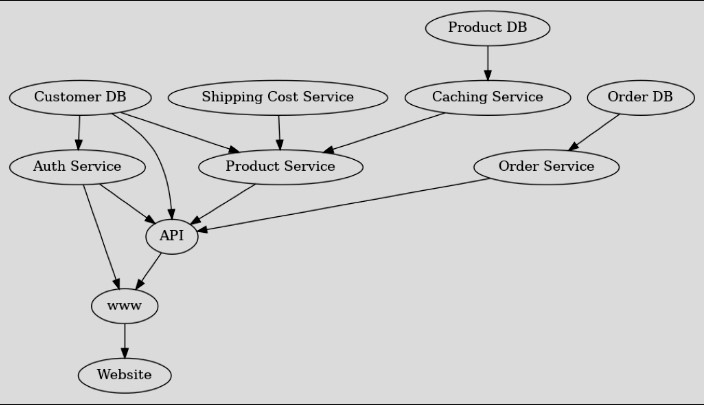
\includegraphics[width=\textwidth]{../copula example/microservice_structurejpg.jpg}
    \caption{Causal DAG for the data.}
    \label{fig:../copula example/microservice_structurejpg.jpg}
\end{figure}


\begin{figure}[h]
    \centering
    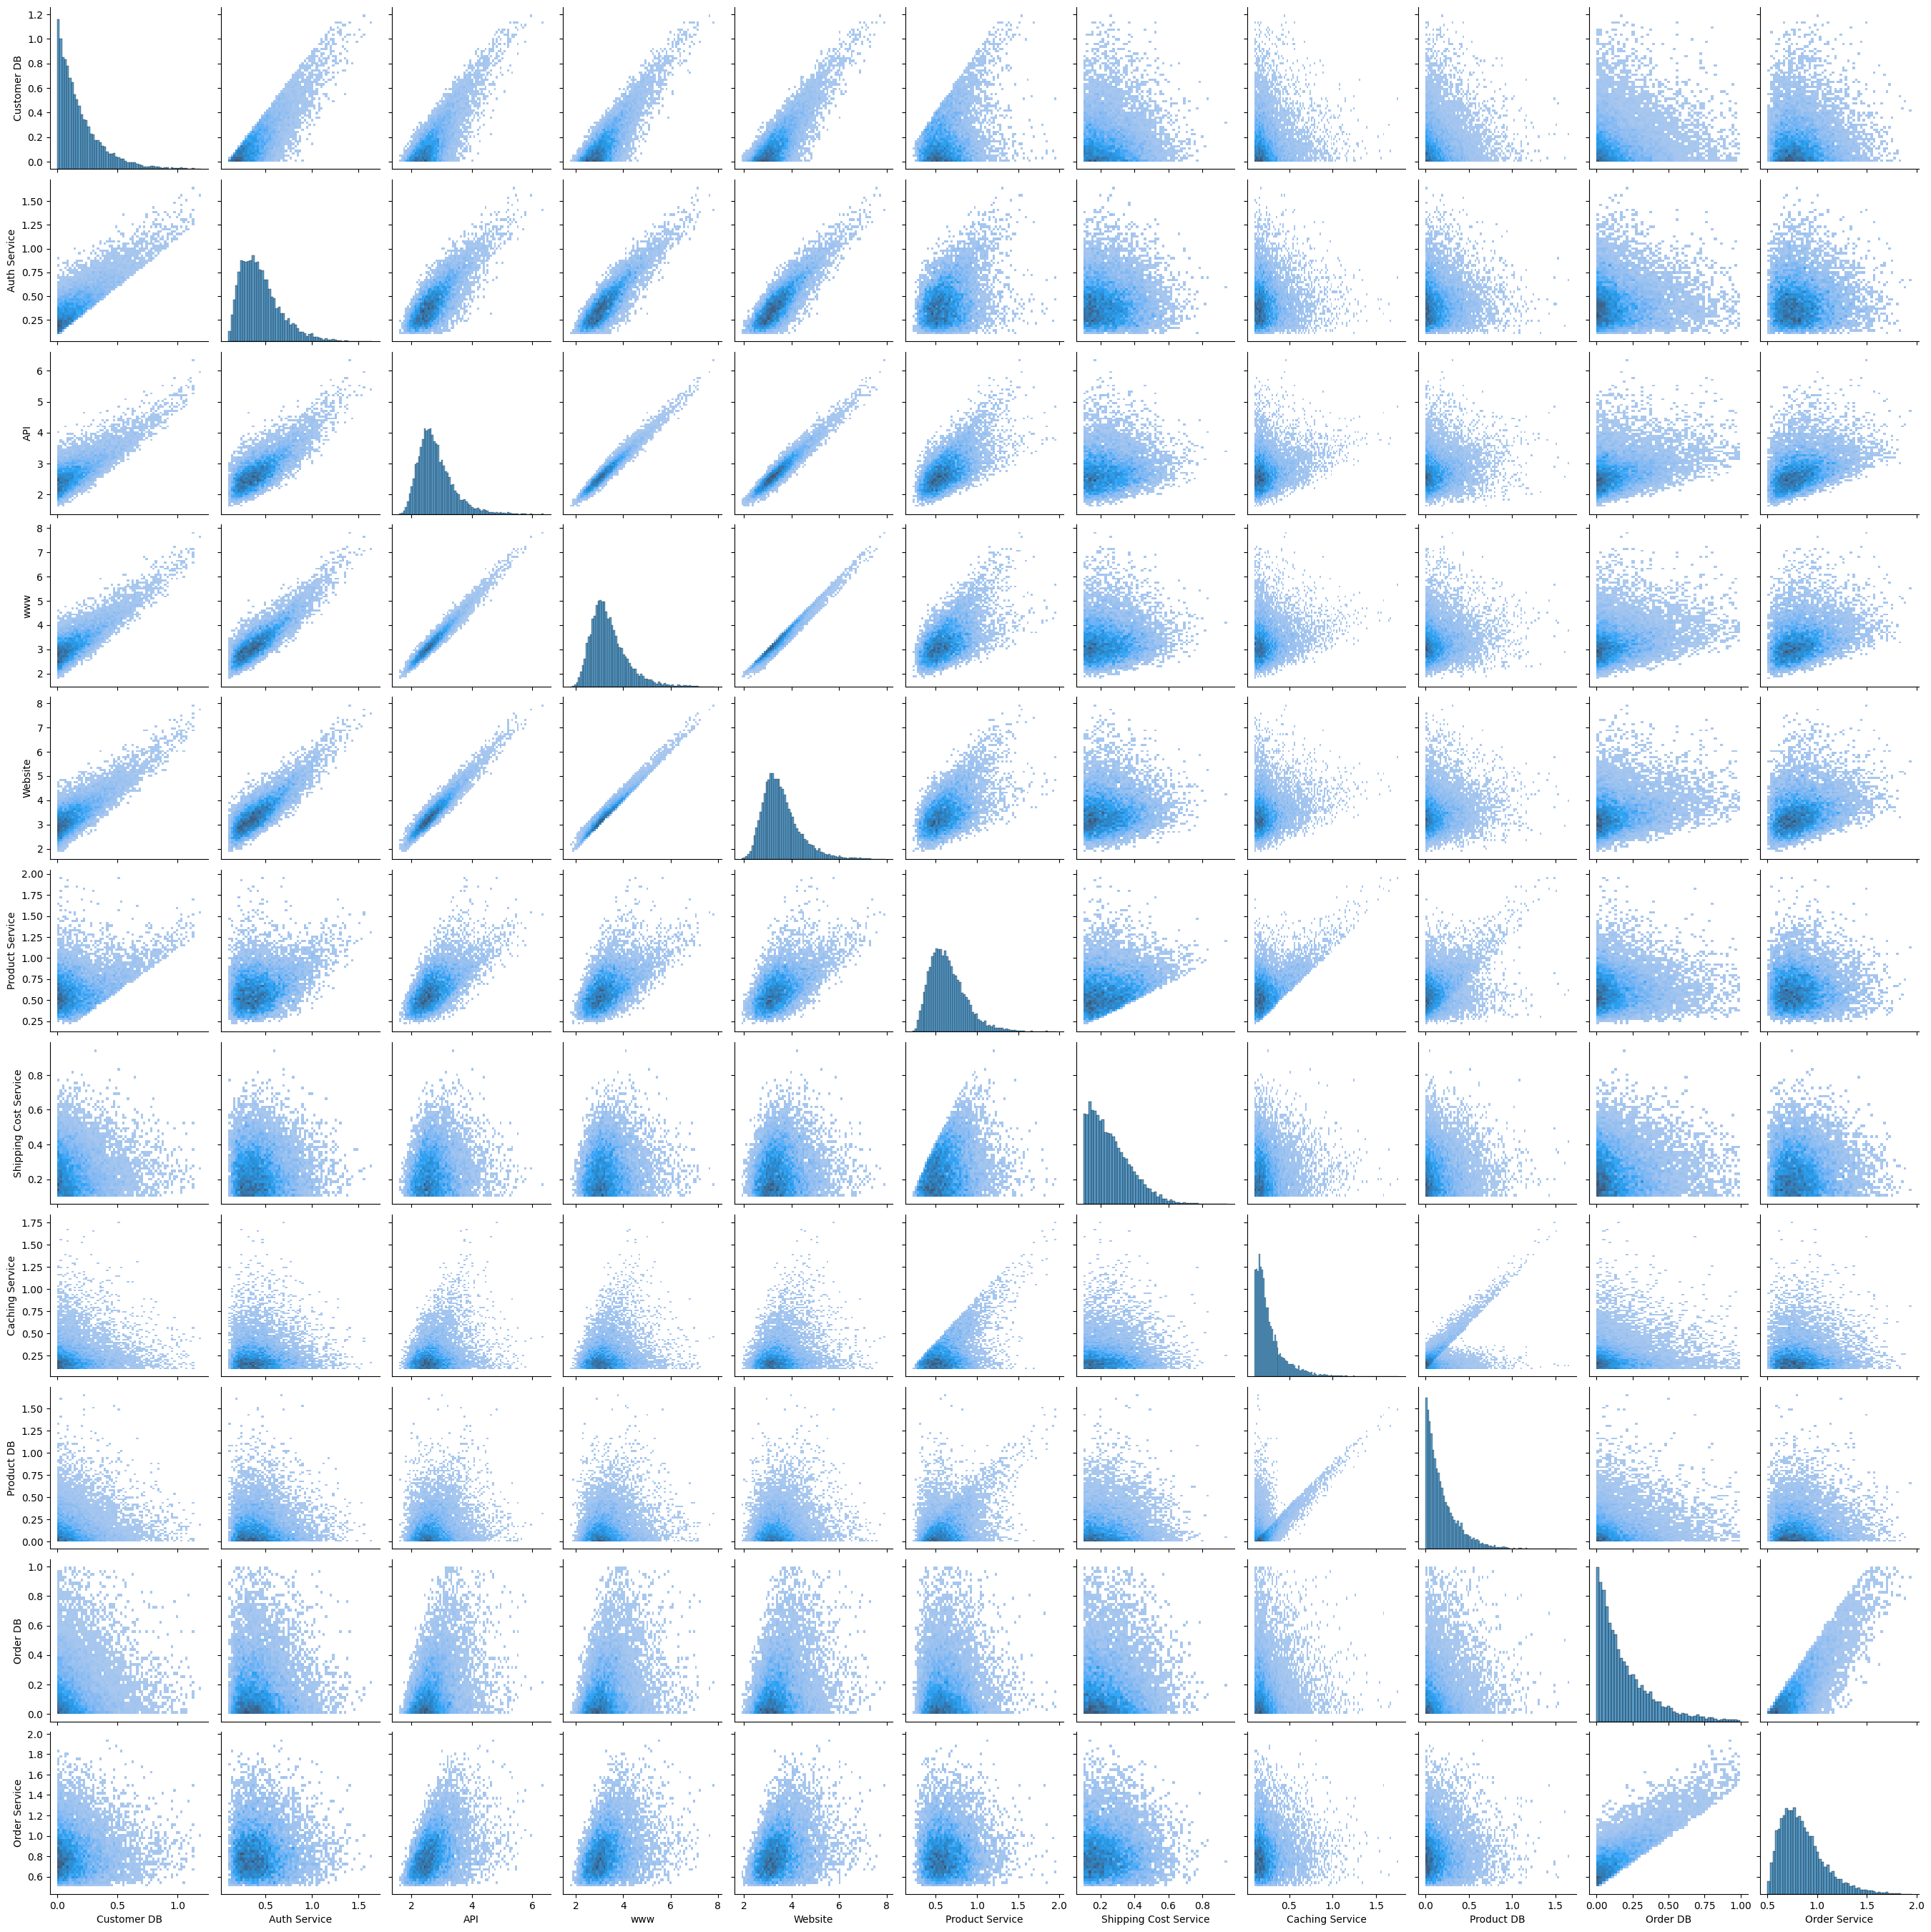
\includegraphics[width=\textwidth]{../copula example/pairplotraw.png}
    \caption{ This a histogram pairplot of the data. This should capture the pairwise dependence structures in the data
        but the non-uniform marginals makes it hard to spot independence, the only obvious dependence structure is
        comonotonicity.}
    \label{fig:rawpairplot}
\end{figure}

\begin{figure}[h]
    \centering
    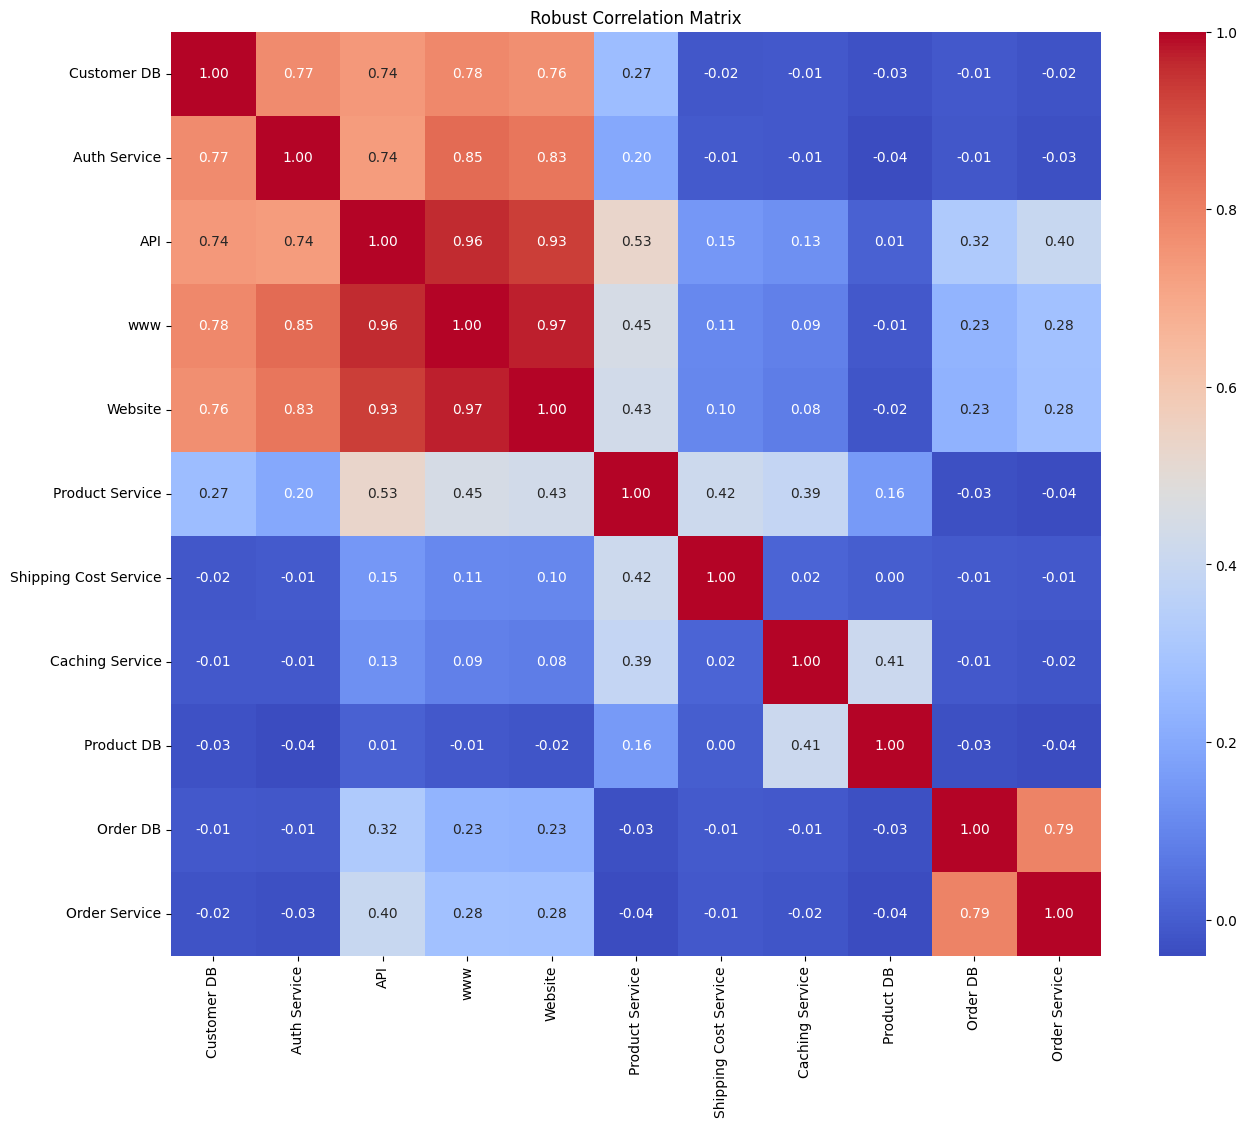
\includegraphics[width=\textwidth]{../copula example/robust_correlation.png}
    \caption{
        This is a heatmap of the robust correlation matrix of the original data. The columns are sorted
        using hdbscan.
    }
    \label{fig:robust correlation}
\end{figure}

\begin{figure}[h]
    \centering
    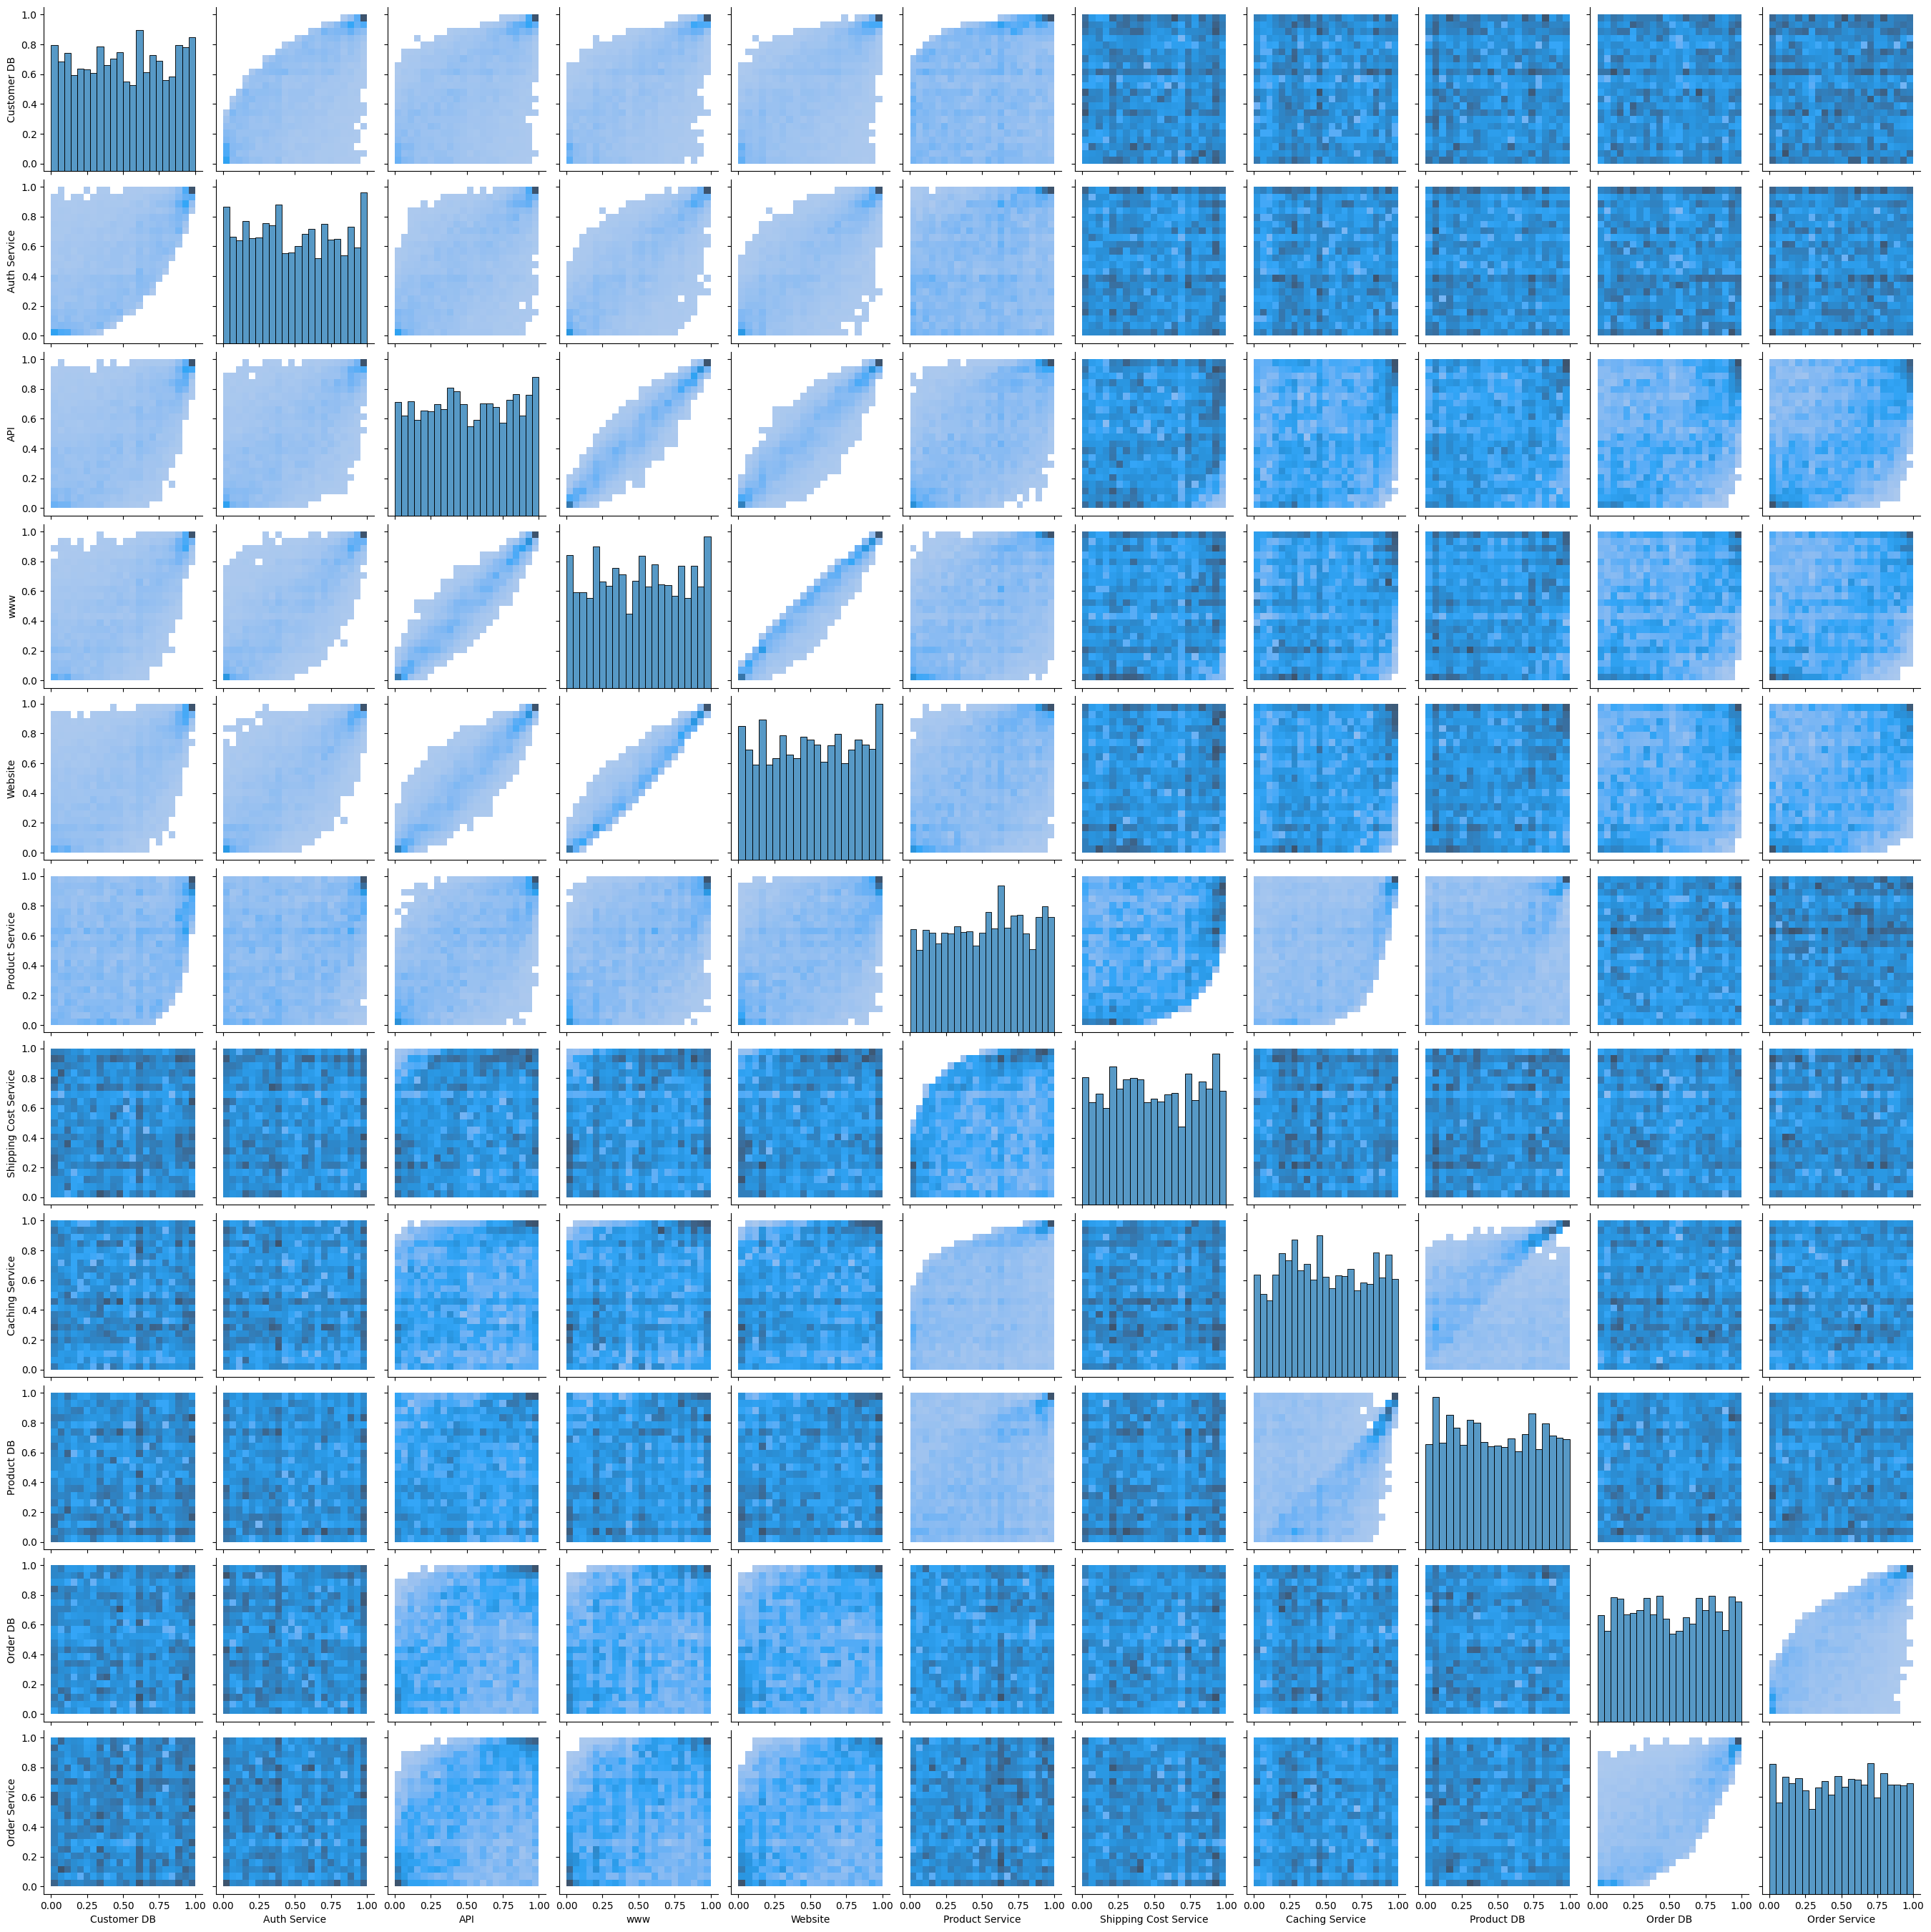
\includegraphics[width=\textwidth]{../copula example/psuedocopulapairplot.png}
    \caption{
        This is a pair plot of psuedo copula samples (marginals are transformed by their sampled emperical cdf).
        Here independence is easily spotted.
    }
    \label{fig:pair plot psuedo copula}
\end{figure}

\newpage
\printbibliography

\end{document}